\chapter{Studie}\label{Studie}
Um das System in der Praxis zu testen, musste im Anschluss eine Nutzerstudie durchgeführt werden.
Dies beinhaltete die Planung und Durchführung der Studie, sowie die Auswertung deren Ergebnisse.
Es musste der Rahmen der Studie geplant und Testpersonen angeworben werden, die darauf einen standardisierten Fragebogen ausfüllen und in einem Interview Fragen beantworten mussten.

\section{Entwurf}\label{Entwurf}
Nachdem die Umsetzung des Bauhausboards Systems abgeschlossen war, galt es einen Test mit Mitarbeitern der Medienfakultät der BUW durchzuführen.
\\
Dafür wurde am Uni-internen Rechenzentrum ein Linux Server mit 2,53GHz Intel Xeon Dualcore, 2GB RAM und Ubuntu Version 14.04 aufgesetzt.
Auf dem Server liefen Node.js, damit Bauhausboards ausgeführt werden konnte und Postfix\footurl{http://www.postfix.org} als Mailserver.
Dieser Mailserver konnte nur Emails an Adressen innerhalb des Universitätsnetzes verschicken, was für die Studie jedoch kein Problem darstellte.
\\
Als Displays wurden neue Tablets angeschafft, die mehr Leistung besaßen, als das Tablet aus der Vorstudie.
Es handelte sich dabei um vier Blaupunkt Discovery 1000c mit 10,1 Zoll Display, 1,33GHz AllWinner A33 Quadcore, 1GB RAM und Android\todotext{4.4 oder 5}. Mit vier Tablets konnten für die Studie vier Räume mit Displays ausgestattet werden.
\\
Damit die Benutzer, wie in der Vorstudie, nicht mit den vorinstallierten Applikationen der Tablets interagieren konnten, musste auch auf den neuen Tablets eine Kiosk-Applikation\footurl{http://www.android-kiosk.com} installiert werden.
\\
Zusätzlich zum Kiosk wurde eine Tasker-App\footurl{http://tasker.dinglisch.net} installiert.
Damit konnte man Aufgaben nach bestimmten Systemereignissen ausführen lassen.
Es wurde Task erstellt, der beim Start des Android-Systems automatisch die Kiosk-App startete, falls das System neu gestartet wurde.
\\
Als Diebstahlsicherung konnte man auf den Tablets Google Locate aktivieren.
Es diente zur Ortung der Geräte, falls diese gestohlen worden wären.
\\
\\
Um die Displays aufhängen zu können, musste eine geeignete Befestigungsmöglichkeit gefunden werden.
Jedoch sollten keine neuen Löcher zur Aufhängung an den Wänden neben den Büros entstehen.
Deswegen sollten die Displays erneut mit Hilfe der bereits aufgehängten Türschilder befestigt werden.
Da bei dieser Studie die Tablets nicht wie in der Vorstudie, durch Löcher in der Tablet-Rückwand, aufgehangen werden konnten, musste die Befestigung anders ausfallen.
Zu diesem Zweck wurden 3D gedruckte Eckstücke \abb{img:Eckstuecke}, mit denen die Tablets befestigt werden konnten, auf eine Plexiglasplatte geschraubt \abb{img:fertigeAufhaengung}.
Diese Aufhängung nutzte die Bohrlöcher für die bereits vorhandenen Türschilder mit, wodurch keinerlei Eingriff in die Bausubstanz entstand.
\\\todotext{Bild von den Eckstücken und von der fertigen Aufhängung}\\
\begin{figure}%[h!]
  \centering
    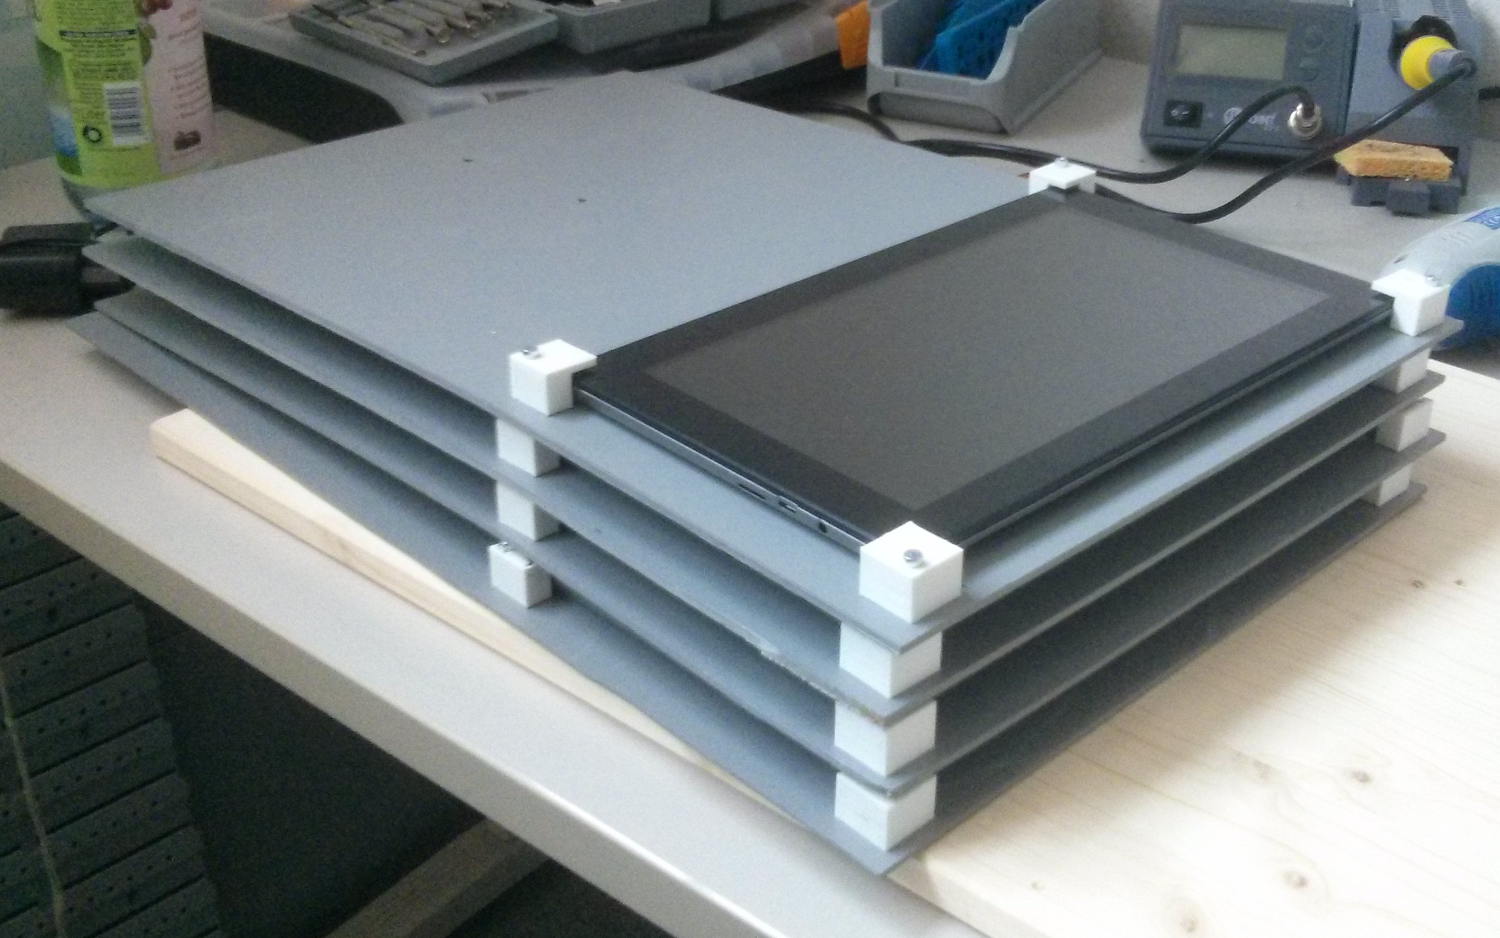
\includegraphics[width=0.85\textwidth]{./img/fertigeAufhaengung.png}
  \caption{Bauhausboards - Aufhängung}
  \label{img:fertigeAufhaengung}
\end{figure}
\\
Damit sich die Testnutzer mit der Grundlegenden Funktion von Bauhausboards vertraut machen konnten, habe ich ein Benutzerhandbuch erstellt.

% Nachdem Umsetzung abgeschlossen war: Test mit echten Nutzern
% Server mit NodeJS und Postfix aufgesetzt
% - Programm auf Server in Uni eingerichtet -> Spezifikationen? oder wurde das schon vorher angegeben?
% - Mailserver installiert, damit Server mails verschicken konnte (nur uni-intern)
% 4 Tablets angeschafft (Durch 4 Tablets -> 4 Räume zum Testen möglich)
%- Blaupunkt Discovery 1000c
%   * 10,1"
%   * CPU: Quadcore @ 1,33GHz
%   * Android 5.1
%   * 1GB RAM
%   * 1024x600 Auflösung (~17:10)
% Alle Tablets mit Kiosk-Mode Browser bestückt
%- Kiosk Mode Browser App auf Tablets um beenden der Bauhausboards App zu verhindern
%- Tasker zum automatischen start des kiosk modes nach systemstart - falls schlaue leute denken, sie können damit den kiosk browser umschiffen
%- Google Locate um Position des Tablets zu bestimmen, im falle eines Diebstahls
%- Rahmen: 4 Tablets -> 4 Räume
%- Wandbefestigung
%  * 3D gedruckte Eckstücke mit Loch um Tablets zu halten + zu sichern
%  * Holz/Blech Rückwand >> plexiglas
%  * Nutzung des vorhandenen Türschildes
%  * Fotos und 3D Model
%- Nutzer Tutorial zur Nutzung des Tools entworfen




\section{Durchführung}\label{Durchführung}
Da nur vier Räume mit Tablets ausgestattet werden konnten, war es von Vorteil, mit den vorhandenen Mitteln möglichst viele Testnutzer organisieren zu können.
Nachdem mehrere verschiedene Leute der Medienfakultät der BUW nach Teilnahme an der Studie gefragt wurden, war es mir möglich einige Mitarbeiter der Professur für Systeme der virtuellen Realität (VR) und der Professur für grafische Datenverarbeitung (CG) zur Teilnahme an der Studie zu bewegen.
\\
Bei der virtuellen Realität gab es drei Büroräume.
Zwei davon mit jeweils drei und einer mit zwei Mitarbeitern.
An der Professur für grafische Datenverarbeitung gab es zwei Mitarbeiter, die sich einen Raum teilten.
Diese Räume befanden sich alle im selben Gang der Fakultät.
\\
Da ein Mitarbeiter der VR Professur durch seine Forschungsarbeit nicht in seinem Büro sein konnte, nahm er nicht an der Studie teil.
\\
Somit konnten insgesamt 9 \todotext{Doktoranden und wie heißen die fertigen Doktoranden?} Testnutzer organisiert werden.
\\
\\
Bevor die Studie beginnen konnte, mussten die Boards angebracht werden.
\\\todotext{Bild von aufgehängten Boards}\\
Außerdem musste eine gute WLAN Verbindung für sie gewährleistet sein.
\\\todotext{Grundriss des Gangs mit Tablets + Accesspoint}\\
Nachdem die Boards aufgehangen waren, wurde für jeden Benutzer ein Account erstellt, die Boards eingerichtet und die Nutzer kurz eingewiesen.
\\
Die Dauer der Studie beschränkte sich auf zwei Wochen.
Damit sollte mindestens ein Wochenende mit eingeplant sein, da sich das Benutzerverhalten nach diesen zwei Tagen ändern konnte.
\\
Während der Studie kam es von Zeit zu Zeit dazu, dass einige Testnutzern Fragen zu bestimmten Funktionen hatten, welche direkt geklärt wurden.
Das System wurde gut genutzt und einige Gäste hinterließen den Testern Nachrichten.
\\\todotext{hier noch weiter auf die vorbeigehenden Nutzer eingehen?}



\section{Auswertung}\label{Auswertung}
% Einfach die Ergebnisse der Studie und wie gut die Boards aufgenommen wurden

%- UEQ Fragebogen nach Testlauf
%- Interview mit allen Testern
%- herausfinden wer so vorbeigehender Nutzer war


%- Aufnahme des Interviews (Audiofile)
%- manche Nutzer haben nichtmal das Tutorial gelesen ...
% - Ein Großteil der Nutzer meinte, dass es unersichtlich ist, wer alles im Raum arbeite und es besser wäre, dass man auf den ersten Blick erkennen könnte, wer alles drin arbeitet (sowas wie Nutzerliste Rechts unter Header)
% - Ein Bug wurde entdeckt, dass wenn man noch keinen Content eingestellt hatte und man dann einen Hintergrund setzen will man ausgeloggt wird, da eine exception geschmissen wurde (Lösung eigene Background Tabelle in der DB)
% - Bei einem User ging nach einer weile der Sidebar nichtmehr (möglicherweise, weil js file nicht vollständig geladen und dadurch der swipe listener nicht feuerte)
% - Die UserImages sind manchmal verzerrt komischerweise



% Durchgegangen:
% - Scholli
% - Banafsheh

Interview:
%%%%%%%%%%%%%%%%%%%%%%%%%%%%%%%%%%%%%%%%%%%%%%%%%%%%%%%%%%%%%%%%%%%%%%%%%%%%%%%%
Nachrichten

erhaltene Nachrichten
- keine ernstgemeinte Nachricht
- Spaßnachrichten (Hallo, Grüße, Guten Tag/Morgen)
- Frage, ob Nutzer im Raum

Ersteller der Nachricht
- Nur bei Nachfrage zu 1 Nachricht
- Freunde/Bekannte (sind darauf direkt ins Büro gekommen - haben gefragt, was ist das und haben sich System erklären lassen)

Nachrichten Bemerkungen
- Schwachpunkt, dass die Nutzer ihre Identität nicht kennzeichnen konnten.
- fast nur anonyme Nachrichten
- ein Nutzer hatte falsche Mailadresse eingetragen -> keine Benachrichtigung

Identität gekennzeichnet
- alle Nachrichten ohne Identität

Alternative Nachrichten Möglichkeit zum Nutzer
- Email
- Telefonisch
- Post-It
- Instant Message
- Mündlich (klopfen)

Einschätzung, ob es anders war, über das Board Nachrichten zu erhalten
- war wie normale mail (war demnacht gut)
- Die Besucher konnten nicht so lange warten, bis Besitzer Nachricht gelesen

Wie schnell die Nachricht gelesen
- schnell

Nachricht im Backend oder per Mail
- per Mail  2
- per backend 0
- ein Nutzer hat keines der beiden genutzt (hat geahnt, dass es diese Funktion gibt)

+/- Nachrichtensystem
+ Zeichnen
+ dass Besucher Besitzer Nachrichten hinterlassen können, wenn der Nicht da ist (besonders gut wenn man kein Handy dabei hat)
- Man konnte nicht sehen, wer die Nachricht geschrieben hat
- Besucher waren nicht gezwungen Identität anzugeben
- zu kompliziert einfach nur einen Text als Nachricht eingeben zu können

Anregungen Nachrichtensystem
- leichtere Textnachrichten
- Voicemail
- Autorkennzeichnung der Nachrichten

Notizen
- gut wenn jemand am Büro ist und niemand da ist, dass er eine Nachricht hinterlassen kann
- ``Wenn es anonym ist, ist es für Besucher spannender und interessanter''
- ``War gut''

%%%%%%%%%%%%%%%%%%%%%%%%%%%%%%%%%%%%%%%%%%%%%%%%%%%%%%%%%%%%%%%%%%%%%%%%%%%%%%%%
Nachrichten verfassen

- die meisten haben nur die Besitzerfunktion wahrgenommen und anderen keine Nachricht auf ihr Board geschrieben
  (vllt auch dadurch, da sie sich alle so persönlich sehen und deswegen miteinander reden können)
- nicht geschafft

%%%%%%%%%%%%%%%%%%%%%%%%%%%%%%%%%%%%%%%%%%%%%%%%%%%%%%%%%%%%%%%%%%%%%%%%%%%%%%%%
Status

genutzt für
- nur am Anfang

genutzt von
- PC 2
- Board 0

Statustexte
- ``busy''

+/- Statussystem
- zu kompliziert
+ gut, dass es unterstützt wird (dieser Nutzer hat es aber nicht wirklich verwendet)
-+ Nutzer hatte neutrale Einstellung zum Statussystem
- man sieht es nicht auf den ersten Blick
+ Nützlich, wenn man weiß, wann der Nutzer bspw wieder da ist

Warum Status nicht geändert
- Nutzer arbeitet meistens im Büro und wechselt nicht oft den Status (jemandem nach außen mitzuteilen, dass er beschäftigt oder weniger beschäftigt ist hat für ihn keine Motivation)
- vergessen

Nutzer würde Status öfter wechseln, wenn es Vordefinierte Statustexte gibt
- ja 0
- nein 1

Nutzung der N/A Funktion
- ja 0
- nein 1

Anregungen Statussystem
- deutlicher Machen

Notizen
- Nutzer war eh die ganze Zeit da und musste dafür keinen Status einstellen
  ``Wenn man nicht da ist, ist es überflüssig, es sei denn man ist wirklich beschäftigt''
- Statusnachricht macht nur dann sinn wenn jemand erwartet wird, dem man gezielt eine Nachricht hinterlassen will (ähnlich wie post-its)
- dachte keiner hat Interesse am Status, Besucher schauen sich nur Bilder an und hinterlassen Nachrichten

%%%%%%%%%%%%%%%%%%%%%%%%%%%%%%%%%%%%%%%%%%%%%%%%%%%%%%%%%%%%%%%%%%%%%%%%%%%%%%%%
Content

genutzt für
- Fachlicher Inhalt (aktuelle Arbeit)
- Spaß
- Gif einfügen
- Bild

genutzt, weil
- Technologie war neu, deswegen rumprobiert (was geht mit dem System)

nicht genutzt, weil
-

üblicherweise Änderungsgrund
- Mittagszeit, da Pausenstimmung
- Am Anfang der Studie

Gäste darauf eingegangen
- ja 1
  * haben geklopft und gefragt ``was ist das?''
- nein 1

+/- Content
+ ``Sehr gut war die Möglichkeit Kreativ zu werden und von der Steuerung und Visuellem selber mit Touch eine Skizze anzufertigen''
+ hat Spaß gemacht
+ ohne Mühe Skizzen erzeugbar

Anregungen
- Mehr Werkzeuge
- Formeln
- Formen

Notizen
- wenn es offiziell da hängen würde: Content mehr offiziell
- Man muss mit dem Editor sehr sorgfältig umgehen, um Skizzen so zu machen, dass sie passen

%%%%%%%%%%%%%%%%%%%%%%%%%%%%%%%%%%%%%%%%%%%%%%%%%%%%%%%%%%%%%%%%%%%%%%%%%%%%%%%%
Backgroundfeature

genutzt
- ja 2
  * für Gif genutzt
  * für Bilder
- nein 0
(alle haben keine extra Seite entworfen)

+/- Background
+ dass man Hintergrund auswählen kann (abhängig vom Vordergrund, was man für eine Skizze macht)
+ war nicht verwirrend
+ viel einfacher, anstatt selber Skizzen zu machen

%%%%%%%%%%%%%%%%%%%%%%%%%%%%%%%%%%%%%%%%%%%%%%%%%%%%%%%%%%%%%%%%%%%%%%%%%%%%%%%%
Twitterfeature

überhaupt Bekannt
- ja 0
- nein 2

hätte Nutzer benutzt?
- ja 0
- nein 2
  * da kein Account 2


%%%%%%%%%%%%%%%%%%%%%%%%%%%%%%%%%%%%%%%%%%%%%%%%%%%%%%%%%%%%%%%%%%%%%%%%%%%%%%%%
Editor

eigene Skizzen gezeichnet
- ja 2
  * eigene Arbeit visualisiert
  * kurze Probe (kleine Zeichnung Text)
- nein 0

Icons
- Teilweise ersichtlich, teilweise nicht
- lieber bewährte Symbole verwenden

Icons nicht ersichtlich
- Eraser
  * sieht aus wie Telefon
- Color
  * ist wie Textwerkzeug
  * besser wäre Farbeimer
- Selector
  * ist wie Stiftwerkzeug
  * besser wäre gestricheltes Kästchen mit Pointer
- Stroke
  * sollten besser 3 Striche sein

Bilder/Gifs eingefügt
- ja 2
- nein 0

+/- Editor
- Drag&Drop war nicht wirklich ersichtlich -> ersichtlich machen (durch Hinweis ``You can also Drop Images'') oder extra Button einfügen
- keine Formen

Notizen
- war cool zu benutzen

%%%%%%%%%%%%%%%%%%%%%%%%%%%%%%%%%%%%%%%%%%%%%%%%%%%%%%%%%%%%%%%%%%%%%%%%%%%%%%%%
Board Allgemein

Backend genutzt
- ja 1
- nein 0

Backend Anmerkungen
- Position im Backend war nicht ersichtlich
- Backend trennen vom Frontend und nicht auf dem Board anbieten (Frontend wäre frei von Overhead)

Passwort + Pin
- Nutzer war verwirrt, warum er zweites Passwort eingeben musste
- Nutzer möchte nur ein Passwort für das ganze Backend und nicht zwei
- Pin als schnelle Authentisierung ist nicht Sinnvoll

Vor-/Nachteile gegenüber Post-Its Whiteboards Pinnwänden
+ man kann digitalen Content erzeugen (Gifs, Bilder)
+ Produziert keinen Müll
+ sofortige Mailbenachrichtigung
  * macht Nachrichten unabhängig vom Ort

Größe der Boards
- genau richtig 1
- zu groß 0
- zu klein 0

regulär Boards weiter zu benutzen
- ja 1
- nein 0

Verbesserungsvorschläge
- Voicemails
- Videomails

Anmerkungen
- Zeitlicher Wechsel zwischen Nutzern war schlecht
  -> lieber Nutzer parallel anzeigen lassen (mit weniger Platz)
  -> wenn man dann jemanden Messagen will soll man denjenigen direkt anwählen können
  -> sofortige Sicht über alle Nutzer im Raum, wer ist grad da, wer ist nicht da, wenn jemand nicht da ist: messsage hinterlassen
  - da meist nicht mehr als 3 Leute in den Büros sitzen wäre 1/3 Platz noch akzeptabel
  - Besucher sehen auf ersten Blick wer da ist und wer nicht
- Studie war zu kurz - Nutzer hatten sich nach 2 Wochen dran gewöhnt (nur leider ist das nicht in komplett in den Arbeitsflow mit eingegangen)
- Menüpunkte schlecht bezeichnet